% Options for packages loaded elsewhere
\PassOptionsToPackage{unicode}{hyperref}
\PassOptionsToPackage{hyphens}{url}
%
\documentclass[
  10pt,
  a4paper,
]{article}
\usepackage{amsmath,amssymb}
\usepackage{iftex}
\ifPDFTeX
  \usepackage[T1]{fontenc}
  \usepackage[utf8]{inputenc}
  \usepackage{textcomp} % provide euro and other symbols
\else % if luatex or xetex
  \usepackage{unicode-math} % this also loads fontspec
  \defaultfontfeatures{Scale=MatchLowercase}
  \defaultfontfeatures[\rmfamily]{Ligatures=TeX,Scale=1}
\fi
\usepackage{lmodern}
\ifPDFTeX\else
  % xetex/luatex font selection
  \setmainfont[]{DejaVu Sans}
  \setmonofont[]{DejaVu Sans Mono}
\fi
% Use upquote if available, for straight quotes in verbatim environments
\IfFileExists{upquote.sty}{\usepackage{upquote}}{}
\IfFileExists{microtype.sty}{% use microtype if available
  \usepackage[]{microtype}
  \UseMicrotypeSet[protrusion]{basicmath} % disable protrusion for tt fonts
}{}
\makeatletter
\@ifundefined{KOMAClassName}{% if non-KOMA class
  \IfFileExists{parskip.sty}{%
    \usepackage{parskip}
  }{% else
    \setlength{\parindent}{0pt}
    \setlength{\parskip}{6pt plus 2pt minus 1pt}}
}{% if KOMA class
  \KOMAoptions{parskip=half}}
\makeatother
\usepackage{xcolor}
\usepackage[margin=19mm]{geometry}
\usepackage{color}
\usepackage{fancyvrb}
\newcommand{\VerbBar}{|}
\newcommand{\VERB}{\Verb[commandchars=\\\{\}]}
\DefineVerbatimEnvironment{Highlighting}{Verbatim}{commandchars=\\\{\}}
% Add ',fontsize=\small' for more characters per line
\newenvironment{Shaded}{}{}
\newcommand{\AlertTok}[1]{\textcolor[rgb]{1.00,0.00,0.00}{\textbf{#1}}}
\newcommand{\AnnotationTok}[1]{\textcolor[rgb]{0.38,0.63,0.69}{\textbf{\textit{#1}}}}
\newcommand{\AttributeTok}[1]{\textcolor[rgb]{0.49,0.56,0.16}{#1}}
\newcommand{\BaseNTok}[1]{\textcolor[rgb]{0.25,0.63,0.44}{#1}}
\newcommand{\BuiltInTok}[1]{\textcolor[rgb]{0.00,0.50,0.00}{#1}}
\newcommand{\CharTok}[1]{\textcolor[rgb]{0.25,0.44,0.63}{#1}}
\newcommand{\CommentTok}[1]{\textcolor[rgb]{0.38,0.63,0.69}{\textit{#1}}}
\newcommand{\CommentVarTok}[1]{\textcolor[rgb]{0.38,0.63,0.69}{\textbf{\textit{#1}}}}
\newcommand{\ConstantTok}[1]{\textcolor[rgb]{0.53,0.00,0.00}{#1}}
\newcommand{\ControlFlowTok}[1]{\textcolor[rgb]{0.00,0.44,0.13}{\textbf{#1}}}
\newcommand{\DataTypeTok}[1]{\textcolor[rgb]{0.56,0.13,0.00}{#1}}
\newcommand{\DecValTok}[1]{\textcolor[rgb]{0.25,0.63,0.44}{#1}}
\newcommand{\DocumentationTok}[1]{\textcolor[rgb]{0.73,0.13,0.13}{\textit{#1}}}
\newcommand{\ErrorTok}[1]{\textcolor[rgb]{1.00,0.00,0.00}{\textbf{#1}}}
\newcommand{\ExtensionTok}[1]{#1}
\newcommand{\FloatTok}[1]{\textcolor[rgb]{0.25,0.63,0.44}{#1}}
\newcommand{\FunctionTok}[1]{\textcolor[rgb]{0.02,0.16,0.49}{#1}}
\newcommand{\ImportTok}[1]{\textcolor[rgb]{0.00,0.50,0.00}{\textbf{#1}}}
\newcommand{\InformationTok}[1]{\textcolor[rgb]{0.38,0.63,0.69}{\textbf{\textit{#1}}}}
\newcommand{\KeywordTok}[1]{\textcolor[rgb]{0.00,0.44,0.13}{\textbf{#1}}}
\newcommand{\NormalTok}[1]{#1}
\newcommand{\OperatorTok}[1]{\textcolor[rgb]{0.40,0.40,0.40}{#1}}
\newcommand{\OtherTok}[1]{\textcolor[rgb]{0.00,0.44,0.13}{#1}}
\newcommand{\PreprocessorTok}[1]{\textcolor[rgb]{0.74,0.48,0.00}{#1}}
\newcommand{\RegionMarkerTok}[1]{#1}
\newcommand{\SpecialCharTok}[1]{\textcolor[rgb]{0.25,0.44,0.63}{#1}}
\newcommand{\SpecialStringTok}[1]{\textcolor[rgb]{0.73,0.40,0.53}{#1}}
\newcommand{\StringTok}[1]{\textcolor[rgb]{0.25,0.44,0.63}{#1}}
\newcommand{\VariableTok}[1]{\textcolor[rgb]{0.10,0.09,0.49}{#1}}
\newcommand{\VerbatimStringTok}[1]{\textcolor[rgb]{0.25,0.44,0.63}{#1}}
\newcommand{\WarningTok}[1]{\textcolor[rgb]{0.38,0.63,0.69}{\textbf{\textit{#1}}}}
\usepackage{longtable,booktabs,array}
\usepackage{calc} % for calculating minipage widths
% Correct order of tables after \paragraph or \subparagraph
\usepackage{etoolbox}
\makeatletter
\patchcmd\longtable{\par}{\if@noskipsec\mbox{}\fi\par}{}{}
\makeatother
% Allow footnotes in longtable head/foot
\IfFileExists{footnotehyper.sty}{\usepackage{footnotehyper}}{\usepackage{footnote}}
\makesavenoteenv{longtable}
\usepackage{graphicx}
\makeatletter
\def\maxwidth{\ifdim\Gin@nat@width>\linewidth\linewidth\else\Gin@nat@width\fi}
\def\maxheight{\ifdim\Gin@nat@height>\textheight\textheight\else\Gin@nat@height\fi}
\makeatother
% Scale images if necessary, so that they will not overflow the page
% margins by default, and it is still possible to overwrite the defaults
% using explicit options in \includegraphics[width, height, ...]{}
\setkeys{Gin}{width=\maxwidth,height=\maxheight,keepaspectratio}
% Set default figure placement to htbp
\makeatletter
\def\fps@figure{htbp}
\makeatother
\setlength{\emergencystretch}{3em} % prevent overfull lines
\providecommand{\tightlist}{%
  \setlength{\itemsep}{0pt}\setlength{\parskip}{0pt}}
\setcounter{secnumdepth}{-\maxdimen} % remove section numbering
\ifLuaTeX
\usepackage[bidi=basic]{babel}
\else
\usepackage[bidi=default]{babel}
\fi
\babelprovide[main,import]{french}
\ifPDFTeX
\else
\babelfont{rm}[]{DejaVu Sans}
\fi
% get rid of language-specific shorthands (see #6817):
\let\LanguageShortHands\languageshorthands
\def\languageshorthands#1{}
\usepackage{etoolbox}
\usepackage{microtype}
\usepackage{float}
\floatplacement{figure}{H}
\setlength{\emergencystretch}{3em}
\setlength{\parskip}{0.35em}
\AtBeginEnvironment{longtable}{\small}
\ifLuaTeX
  \usepackage{selnolig}  % disable illegal ligatures
\fi
\IfFileExists{bookmark.sty}{\usepackage{bookmark}}{\usepackage{hyperref}}
\IfFileExists{xurl.sty}{\usepackage{xurl}}{} % add URL line breaks if available
\urlstyle{same}
\hypersetup{
  pdflang={fr-FR},
  hidelinks,
  pdfcreator={LaTeX via pandoc}}

\author{}
\date{}

\begin{document}

\hypertarget{v6.42---un-pli-certifiuxe9-sa-paire-et-la-porte-arithmuxe9tique}{%
\section{V6.42 - Un pli certifié, sa paire et la porte
arithmétique}\label{v6.42---un-pli-certifiuxe9-sa-paire-et-la-porte-arithmuxe9tique}}

\textbf{Document 66 · Vincent P. P. NOËL · 12 octobre 2026}

Dossier de recherche, preuves auxiliaires, certificat calculatoire et
source LaTeX.

\hypertarget{la-suite-a-uxe9tuxe9-exuxe9cutuxe9e-un-passage-local-est-maintenant-validuxe9}{%
\subsection{1. La suite a été exécutée : un passage local est maintenant
validé}\label{la-suite-a-uxe9tuxe9-exuxe9cutuxe9e-un-passage-local-est-maintenant-validuxe9}}

\textbf{La famille exacte V13 choisie possède un pli critique double
unique dans la boîte fixée.} Le contrôle de Rouché couvre le contour
continu et tout le petit intervalle radial : il contient exactement deux
zéros avec multiplicité. Aux paramètres \(r_*\pm10^{-4}\), quatre boîtes
de racines sont validées uniformément malgré l'incertitude sur \(r_*\) :
deux zéros critiques avant, une paire hors droite après.

Ce résultat dépasse un accord entre précisions : une borne analytique du
reste, une inclusion stricte et une contraction fournissent existence et
unicité. Le calcul repose sur le backend d'intervalles explicité ; une
validation indépendante de tout ce backend n'est pas revendiquée.

\begin{longtable}[]{@{}
  >{\raggedright\arraybackslash}p{(\columnwidth - 4\tabcolsep) * \real{0.3333}}
  >{\raggedright\arraybackslash}p{(\columnwidth - 4\tabcolsep) * \real{0.3333}}
  >{\raggedright\arraybackslash}p{(\columnwidth - 4\tabcolsep) * \real{0.3333}}@{}}
\toprule\noalign{}
\begin{minipage}[b]{\linewidth}\raggedright
Point
\end{minipage} & \begin{minipage}[b]{\linewidth}\raggedright
Résultat V6.42
\end{minipage} & \begin{minipage}[b]{\linewidth}\raggedright
Portée
\end{minipage} \\
\midrule\noalign{}
\endhead
\bottomrule\noalign{}
\endlastfoot
Pli sélectionné & Validations à 50 puis 80 décimales & Même boîte et
même recette ; projection réelle non nulle \\
Contour & 256 arcs, comparaison stricte de Rouché & Cercle continu, pour
tout r du petit intervalle \\
Quatre racines & Quatre contractions uniformes et boîtes disjointes &
Deux critiques par symétrie et unicité ; deux hors droite \\
Paire et opérateur & Signature locale certifiée avant et après & Pas de
métrique positive non dégénérée au point double \\
Porte globale & Forme arithmétique et inégalité uniforme explicites & Le
signe de la forme complète demeure ouvert \\
\end{longtable}

\textbf{Une voie est fermée précisément.} Toute métrique hermitienne
positive symétrisant le compagnon réel exige μ\textgreater0. Elle
dégénère ou devient non uniformément bornée à l'approche du pli ; au
double, le bloc de Jordan interdit une métrique définie positive. C'est
une impossibilité locale, pas une impossibilité de prouver RH.

La cible RH et les deux portes globales gardent leur portée : le
certificat ne fournit ni le signe de Weil pour tous les tests, ni une
borne suffisante sur l'énergie arithmétique Q(X). Il certifie une
composante choisie de V13. Dans cette continuation radiale,
\(A=\cos r\,z_i\) varie ; le déploiement sur une fibre à A constant
reste une expérience distincte.

\newpage

\hypertarget{encadrements-marges-et-sens-de-la-preuve}{%
\subsection{2. Encadrements, marges et sens de la
preuve}\label{encadrements-marges-et-sens-de-la-preuve}}

Le protocole sélectionne, parmi les six plis attribués V6.41, celui de
plus petite hauteur absolue : \texttt{fold\_k1\_plus\_5}, famille
\texttt{k1\_rpi\_6}, membre plus. Les centres rationnels sont
\(r_0=0,243079394165\) et \(t_0=4,861023490998\), avec demi-largeur
\(10^{-9}\). Le verrou est antérieur à toute nouvelle évaluation de
fonction L.

\begin{longtable}[]{@{}ll@{}}
\toprule\noalign{}
Contrôle & Valeur ou encadrement certifié \\
\midrule\noalign{}
\endhead
\bottomrule\noalign{}
\endlastfoot
r* & {[}0.243079394165044055784476 ; 0.243079394165045645672933{]} \\
t* & {[}4.861023490998065424261169 ; 4.861023490998073695541661{]} \\
κ=−2 Hr/Htt & {[}-1.807995896101449197 ; -1.807983145236999804{]} \\
Contraction du pli, 50 décimales & q ≤ 0.000002849667 \textless{} 1 \\
Contraction du pli, 80 décimales & q ≤ 0.000004135641 \textless{} 1 \\
Module de comparaison sur le cercle & ≥ 0.0437791153 \\
Majorant du défaut sur les 256 arcs & ≤ 0.0303866506 \\
Marge uniforme de Rouché & ≥ 0.0133924647 \textgreater{} 0 \\
\end{longtable}

Les décimales affichées du tableau sont des résumés. Les bornes
complètes et les endpoints binaires, exportés vers l'extérieur, figurent
dans le certificat JSON. Les quatre encadrements ci-dessous sont
volontairement élargis pour une lecture simple :

\begin{longtable}[]{@{}
  >{\raggedright\arraybackslash}p{(\columnwidth - 4\tabcolsep) * \real{0.3333}}
  >{\raggedright\arraybackslash}p{(\columnwidth - 4\tabcolsep) * \real{0.3333}}
  >{\raggedright\arraybackslash}p{(\columnwidth - 4\tabcolsep) * \real{0.3333}}@{}}
\toprule\noalign{}
\begin{minipage}[b]{\linewidth}\raggedright
Paramètre
\end{minipage} & \begin{minipage}[b]{\linewidth}\raggedright
Re(s)
\end{minipage} & \begin{minipage}[b]{\linewidth}\raggedright
Encadrement de Im(s)
\end{minipage} \\
\midrule\noalign{}
\endhead
\bottomrule\noalign{}
\endlastfoot
r*−10⁻⁴, racine haute & 1/2 exactement & {[}4,874488964703 ;
4,874488964747{]} \\
r*−10⁻⁴, racine basse & 1/2 exactement & {[}4,847596737039 ;
4,847596737084{]} \\
r*+10⁻⁴, racine gauche & {[}0,486553813589 ; 0,486553813637{]} &
{[}4,861004131596 ; 4,861004131643{]} \\
r*+10⁻⁴, racine droite & {[}0,513446186366 ; 0,513446186408{]} &
{[}4,861004131599 ; 4,861004131641{]} \\
\end{longtable}

La criticité des deux premières ne vient pas d'un intervalle étroit
autour de 1/2 : chaque boîte est invariante par
\(s\mapsto1-\overline s\), et son zéro unique est donc fixé par la
symétrie fonctionnelle. Les deux autres boîtes excluent la droite
critique. Les quatre localisations sont uniformes pour les intervalles
de paramètres contenant les valeurs exactes \(r_*\pm10^{-4}\).

\begin{figure}
\centering
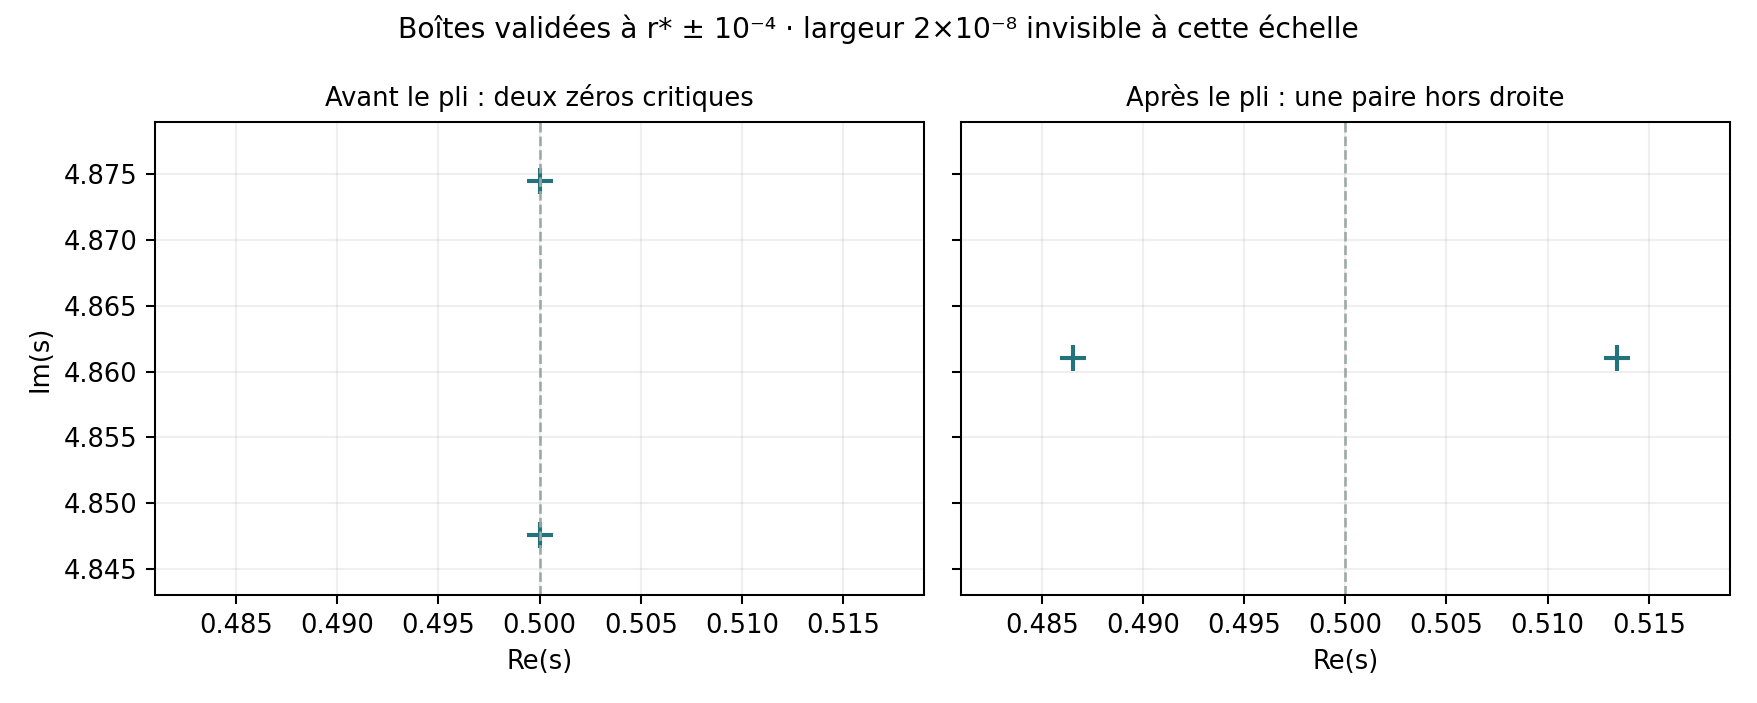
\includegraphics{66_Paire_certifiee.png}
\caption{Deux configurations certifiées de la même paire. Les centres
sont marqués ; les boîtes de validation ont largeur 2×10⁻⁸ et sont
invisibles à cette échelle.}
\end{figure}

\begin{figure}
\centering
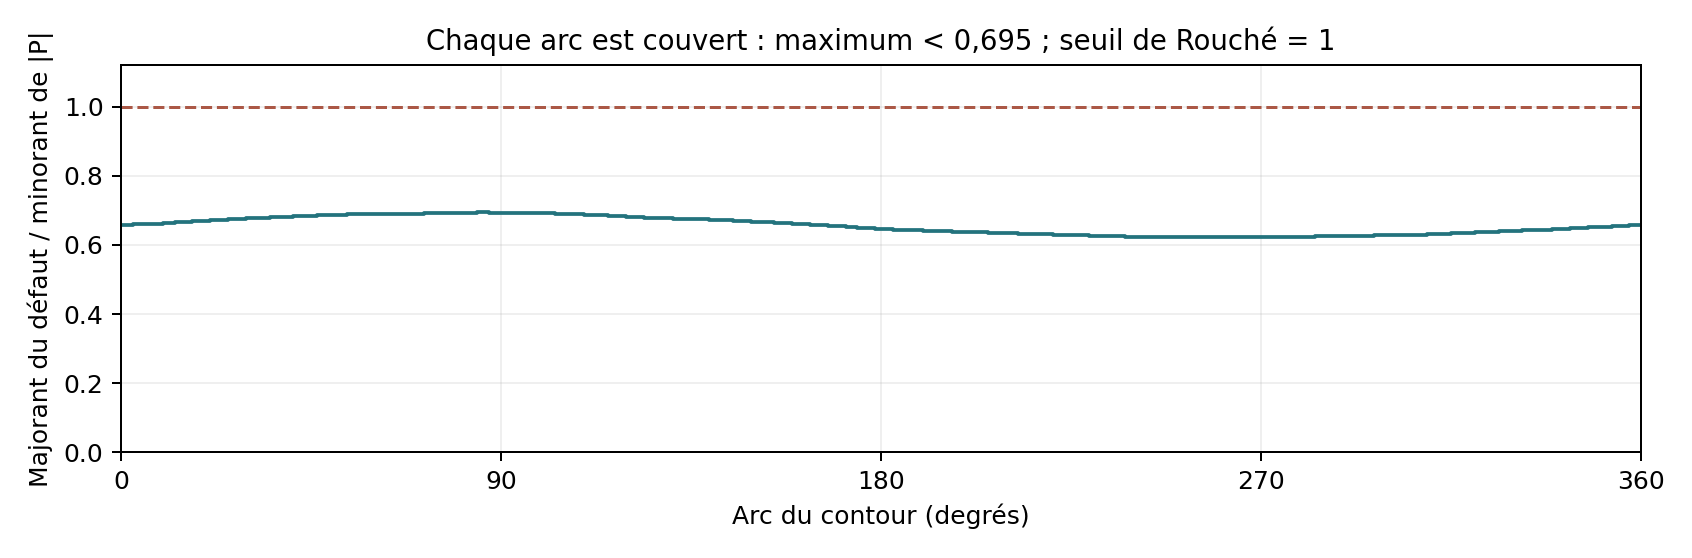
\includegraphics{66_Controle_du_contour.png}
\caption{Majorants sur les 256 arcs : la borne inclut tous les points de
chaque arc et tout le petit intervalle radial. Ce tracé représente une
borne, pas des échantillons du module exact.}
\end{figure}

Une précision de travail de 80 décimales ne signifie pas 80 décimales
certifiées sur les coordonnées. La dépendance des intervalles dans une
boîte de largeur fixée reste dominante. Les encadrements obtenus sont
ceux du tableau et des données, avec leurs marges réellement calculées.

\newpage

\hypertarget{le-graphe-courant-des-acquis-et-des-obstacles}{%
\subsection{3. Le graphe courant des acquis et des
obstacles}\label{le-graphe-courant-des-acquis-et-des-obstacles}}

\begin{figure}
\centering
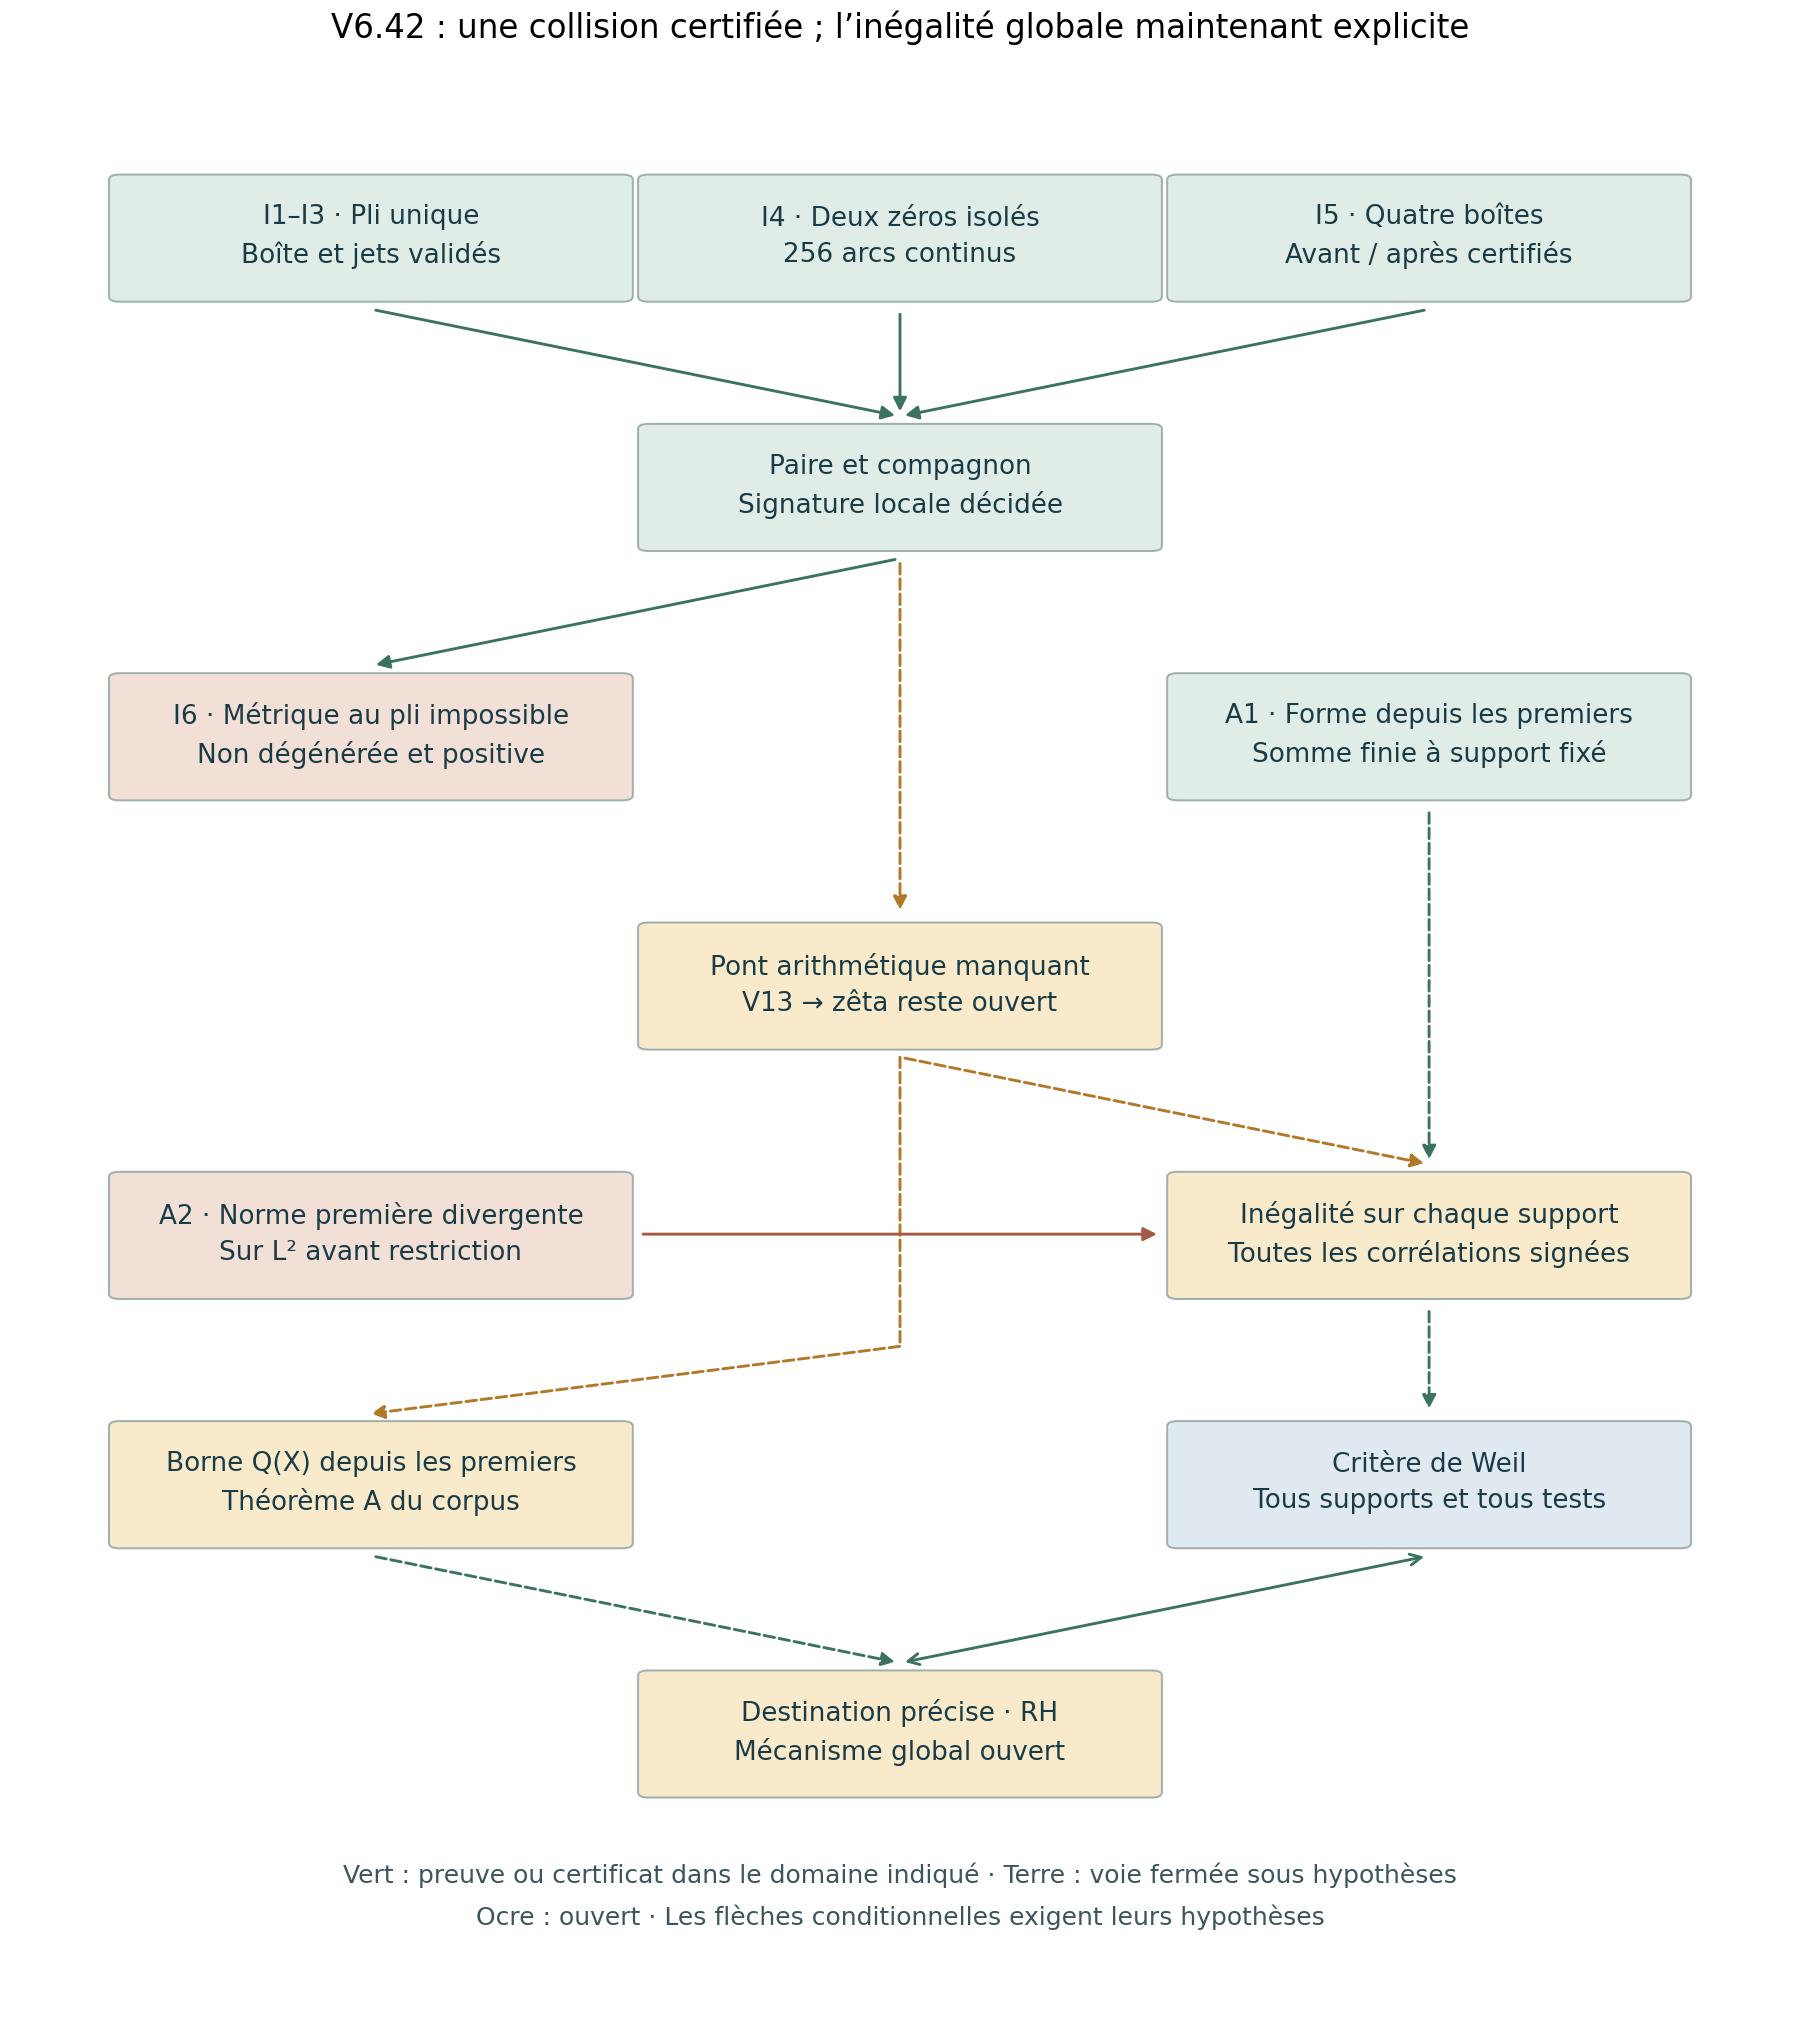
\includegraphics[width=0.85\textwidth,height=\textheight]{66_Graphe_des_certificats.png}
\caption{Un pli et une paire sont validés ; le compagnon rencontre une
impossibilité de métrique au double ; les deux portes arithmétiques
globales restent ouvertes.}
\end{figure}

Le lecteur interactif \texttt{66\_GRAPHE\_DES\_CERTIFICATS.html} relie
chaque nœud à ses preuves et à ses hypothèses. Le graphe historique du
document 65 est conservé. L'observation des 20 candidats V6.41 n'est pas
transformée en une certification des 20 : seul le pli sélectionné reçoit
ce nouveau statut.

\newpage

\hypertarget{duxe9monstrations-locales-et-limites-du-compagnon}{%
\subsection{4. Démonstrations locales et limites du
compagnon}\label{duxe9monstrations-locales-et-limites-du-compagnon}}

\hypertarget{objet-exact-et-suxe9lection-avant-calcul}{%
\subsubsection{1. Objet exact et sélection avant
calcul}\label{objet-exact-et-suxe9lection-avant-calcul}}

Le verrou V6.42 reprend la recette Gauss/minor de \texttt{k1\_rpi\_6},
membre plus. Parmi les six plis attribués de V6.41, la règle choisit
celui de plus petite hauteur absolue, \texttt{fold\_k1\_plus\_5}. Les
quatre graines de racines proviennent des sorties V6.41. Aucun nouveau
support, rayon de contour ou centre n'est choisi selon une issue
favorable.

La fonction est exactement \(F(r,s)=\cos r\,f_i(s)+\sin r\,f_u(s)\), où
\(f_i=z_iL(s,\chi_i)\) et \(f_u=\sum u_jz_jL(s,\chi_j)\). Les \(u_j\)
sont les mineurs normalisés avec l'orientation du manifeste ; ils sont
réels, de norme un, et \(\sum u_jz_j=0\) par l'identité des mineurs. Le
rayon varie : \(A=\cos r\,z_i\) varie aussi. Ce travail ne déploie pas
encore un pli sur une fibre à A constant.

\hypertarget{lemme-i1---un-reste-analytique-et-ses-duxe9rivuxe9es-sont-bornuxe9s}{%
\subsubsection{2. Lemme I1 - Un reste analytique et ses dérivées sont
bornés}\label{lemme-i1---un-reste-analytique-et-ses-duxe9rivuxe9es-sont-bornuxe9s}}

Pour \(a>0\), \(s\ne1\) et \(\sigma+2M>1\), Euler-Maclaurin donne

\[
\begin{aligned}
\zeta(s,a)={}&\sum_{n=0}^{N-1}(n+a)^{-s}
+{(N+a)^{1-s}\over s-1}+\tfrac12(N+a)^{-s}\\
&+\sum_{k=1}^M {B_{2k}\over(2k)!}(s)_{2k-1}(N+a)^{1-s-2k}
+R_{N,M}(s,a).
\end{aligned}
\]

La série de Fourier des Bernoulli périodiques donne
\(|\widetilde B_{2M}(x)|/(2M)!\le2\zeta(2M)/(2\pi)^{2M}\). L'intégrale
du reste implique donc

\[
|R_{N,M}(s,a)|\le
{2\zeta(2M)\over(2\pi)^{2M}}
{|(s)_{2M}|(N+a)^{1-\sigma-2M}\over\sigma+2M-1}.
\]

\textbf{Preuve.} Prendre le module dans l'intégrale du Bernoulli
périodique contre \((s)_{2M}(x+a)^{-s-2M}\), puis intégrer
\((x+a)^{-\sigma-2M}\) depuis N. Tous les facteurs sont explicitement
majorés ; \(\zeta(2M)\le1+1/(2M-1)\) résulte du test intégral. □

Dans le rectangle déclaré, étendu d'une marge \(\delta=1/8\), chaque
facteur \(|s+j|\) est majoré à partir des bornes réelles et imaginaires.
Pour une série périodique de période 13,
\(L(s)=13^{-s}\sum_{a=1}^{12}T_a\zeta(s,a/13)\), la somme des modules
des \(T_a\) et \(13^{-\sigma}\) donnent un majorant R du reste sur ce
rectangle étendu. La formule de Cauchy donne ensuite

\[
|\partial_s^k R_L(s)|\le k!R/\delta^k,\qquad k=0,1,2.
\]

Ces majorants s'ajoutent, dans les deux composantes, aux expressions
finies des jets. Une petite différence entre deux précisions n'est pas
utilisée à la place du reste. Les Bernoulli sont calculés par une
récurrence rationnelle. Les logarithmes portent sur des entiers positifs
; les exponentielles complexes utilisent seulement exp, cos et sin réels
avec intervalles.

Sources primaires des identités {[}Dlm26{]} :
\href{https://dlmf.nist.gov/25.11.iii}{DLMF 25.11(iii)} et
\href{https://dlmf.nist.gov/24.8.i}{DLMF 24.8(i)}. Les majorations
ci-dessus sont explicitées ici séparément.

\hypertarget{lemme-i2---une-projection-ruxe9elle-fixe-pruxe9serve-le-pli}{%
\subsubsection{3. Lemme I2 - Une projection réelle fixe préserve le
pli}\label{lemme-i2---une-projection-ruxe9elle-fixe-pruxe9serve-le-pli}}

L'équation fonctionnelle commune donne sur la droite critique
\(F(r,1/2+it)=e^{-i\theta(t)}Z(r,t)\), avec Z réel analytique. Pour un
complexe constant \(\omega\), poser
\(H(r,t)=\Re[\omega F(r,1/2+it)]=h(t)Z(r,t)\),
\(h(t)=\Re[\omega e^{-i\theta(t)}]\).

Si \(\Re[\omega f_i(1/2+it)]\) est séparé de zéro sur la boîte de
hauteur, h ne s'annule pas : ce terme est \(h(t)Z_i(t)\). Alors

\[
H=H_t=0\iff Z=Z_t=0,
\quad H_r=hZ_r,\quad H_{tt}=hZ_{tt}
\quad\text{au zéro double}.
\]

\textbf{Preuve.} Diviser H par h ; au zéro de Z, dériver une première
fois, puis au zéro de \(Z_t\) une seconde fois. La dérivée radiale ne
dérive pas h. La projection d'ancre non nulle sépare simultanément h et
\(Z_i\) de zéro. □

Ainsi \(\kappa=-2H_r/H_{tt}=-2Z_r/Z_{tt}\). Les jets du système réel
\(G=(H,H_t)\) sont évalués directement depuis \(F,F_s,F_{ss}\) ; aucun
jet Gamma n'est évalué par intervalles. Une non-annulation de \(H_{tt}\)
prouve aussi que le zéro de F en s est exactement double. Les phases
exactes et le facteur Gamma commun justifient l'équation fonctionnelle
employée.

\hypertarget{thuxe9oruxe8me-i3---inclusion-et-contraction-donnent-existence-et-unicituxe9}{%
\subsubsection{4. Théorème I3 - Inclusion et contraction donnent
existence et
unicité}\label{thuxe9oruxe8me-i3---inclusion-et-contraction-donnent-existence-et-unicituxe9}}

Soit une boîte réelle B de centre rationnel \(x_0\), et C une matrice
rationnelle inversible. Soient des intervalles contenant \(G(x_0)\) et
chaque entrée de \(DG(B)\). Définir

\[
K=x_0-CG(x_0)+(I-CDG(B))(B-x_0).
\]

Si \(K\subset\operatorname{int}B\) et \(q=\sup\|I-CDG(B)\|_\infty<1\), G
possède exactement un zéro dans B.

\textbf{Preuve.} Pour \(T(x)=x-CG(x)\), la formule intégrale de la
valeur moyenne donne \(T(B)\subset K\subset B\). La même borne
matricielle donne \(\|T(x)-T(y)\|_\infty\le q\|x-y\|_\infty\) sur B. La
boîte est complète ; le théorème du point fixe fournit une unique
solution de \(T(x)=x\). C étant inversible, elle équivaut à \(G(x)=0\).
Toute solution appartient à K. □

La borne q est la somme maximale des modules des entrées d'une ligne.
Les inclusions sont strictes, comparées comme fractions exactes aux
bornes rationnelles. Le préconditionneur provient de l'inverse rationnel
d'un jacobien arrondi selon la règle fixée ; il n'a pas besoin d'être un
inverse exact du vrai jacobien.

La même démonstration s'applique uniformément pour un paramètre r dans
un intervalle : pour chaque r, \(T_r\) conserve la boîte et possède la
même borne de contraction. Pour un zéro complexe de F, le jacobien réel
est \(\begin{pmatrix}\Re F_s&-\Im F_s\\\Im F_s&\Re F_s\end{pmatrix}\).

\hypertarget{lemme-i4---rouchuxe9-contruxf4le-le-contour-continu-et-tout-le-paramuxe8tre}{%
\subsubsection{5. Lemme I4 - Rouché contrôle le contour continu et tout
le
paramètre}\label{lemme-i4---rouchuxe9-contruxf4le-le-contour-continu-et-tout-le-paramuxe8tre}}

Prendre \(w=-i(s-1/2)\), \(w_0=t_0\) et le cercle \(|w-w_0|=R=1/5\).
Choisir un complexe rationnel non nul α et \(P(w)=\alpha(w-w_0)^2\).
Écrire \(D=F-P\). Sur un arc de milieu \(w_m\) et de distance maximale
d,

\[
|D(w)|\le |D(w_m)|+|D_w(w_m)|d+\tfrac12 B_2d^2,
\quad B_2\ge\sup|D_{ww}|.
\]

\textbf{Preuve.} La formule de Taylor avec reste intégral sur le segment
de \(w_m\) à w donne l'inégalité. Le segment reste dans le disque,
couvert par le rectangle déclaré. Pour n arcs égaux,
\(d=2R\sin(\pi/(2n))\). Les jets sont majorés pour tout r de
l'intervalle. Si chaque majorant est strictement inférieur à
\(|\alpha|R^2\), Rouché donne exactement deux zéros, avec multiplicité,
pour chaque r. □

Le cercle entier est couvert, pas seulement ses points de grille. La
borne de dérivée seconde complète le calcul aux milieux des arcs.
L'absence de pôle dans le disque est justifiée par l'analyticité des
fonctions L et, même sans leur cancellation globale, par l'absence de
s=1 dans ce disque.

\hypertarget{lemme-i5---symuxe9trie-et-unicituxe9-duxe9cident-critique-ou-hors-droite}{%
\subsubsection{6. Lemme I5 - Symétrie et unicité décident critique ou
hors
droite}\label{lemme-i5---symuxe9trie-et-unicituxe9-duxe9cident-critique-ou-hors-droite}}

Pour r réel, l'équation fonctionnelle associe à un zéro s son partenaire
\(1-\overline s\), avec facteurs de complétion non nuls dans les boîtes.
Si une boîte centrée en \(\Re s=1/2\) est invariante par cette symétrie
et contient un zéro unique, ce zéro est critique : son partenaire est le
même. Si une boîte exclut la droite critique, son zéro validé est hors
droite.

\textbf{Preuve.} Le partenaire appartient à la même boîte invariante et
est un zéro ; l'unicité impose \(s=1-\overline s\). Le second cas est
immédiat. □

Deux boîtes disjointes incluses dans le cercle, avec les deux zéros
uniques, identifient toute la paire locale lorsque le compte de Rouché
vaut deux. On peut donc certifier le changement de configuration aux
deux paramètres \(r_*\pm10^{-4}\), même si \(r_*\) est fourni par un
encadrement.

\hypertarget{portuxe9e-de-la-certification-et-vuxe9rifications}{%
\subsubsection{7. Portée de la certification et
vérifications}\label{portuxe9e-de-la-certification-et-vuxe9rifications}}

Le certificat calculatoire repose sur les majorants analytiques
démontrés, les recettes exactes, et le backend mpmath 1.3.0
d'arithmétique élémentaire par intervalles. La documentation qualifie
son support d'expérimental : aucune validation indépendante de tout le
backend n'est présupposée. Le constructeur de copie iv.mpc et
l'involution complexe non supportés sont évités ; les correctifs
d'implémentation restent datés dans les données. Les formules de jets
sont recoupées avec Hurwitz en haute précision, avec le même backend :
ce contrôle est distinct du majorant analytique.

Un vérificateur rationnel relit séparément les intervalles du
certificat, recalcule inclusion, contraction et critères géométriques.
Il vérifie le calcul fini des inégalités ; il ne remplace pas une
réévaluation indépendante des primitives transcendantales. Les sorties
et les refus des plans fixés sont conservés.

Ce certificat concerne une famille V13, un pli, un contour et quatre
boîtes. Il ne certifie pas le premier zéro global, toutes les collisions
ou la positivité arithmétique de ζ. La métrique du compagnon dépend du
discriminant de la paire ; elle ne donne toujours pas le signe global de
la forme de Weil.

\hypertarget{thuxe9oruxe8me-i6---obstacle-uxe0-toute-muxe9trique-positive-du-compagnon-au-pli}{%
\subsubsection{8. Théorème I6 - Obstacle à toute métrique positive du
compagnon au
pli}\label{thuxe9oruxe8me-i6---obstacle-uxe0-toute-muxe9trique-positive-du-compagnon-au-pli}}

Fixer l'unité de hauteur pour rendre les coordonnées adimensionnées.
Pour \(H=\begin{pmatrix}a&1\\\mu&a\end{pmatrix}\) réel, une matrice
symétrique \(G=\begin{pmatrix}p&q\\q&r\end{pmatrix}\) vérifie
\(H^TG=GH\) si et seulement si \(p=\mu r\). Un tel G défini positif
existe si et seulement si \(\mu>0\).

\textbf{Preuve.} La multiplication impose \(p=\mu r\). La positivité
exige \(r>0\) et \(pr-q^2=\mu r^2-q^2>0\), donc \(\mu>0\).
Réciproquement, \(G=\operatorname{diag}(\mu,1)\) convient. □

Pour une métrique hermitienne complexe, l'équation impose également
\(q=\overline q\) ; le même calcul couvre donc ce cas.

Pour \(0<\mu\le1\), le rapport des valeurs propres de G est au moins
\(r/p=1/\mu\), par les quotients de Rayleigh sur les vecteurs de base.
Si \(cI\le G\le CI\), on a \(\mu=p/r\ge c/C\). Une métrique uniformément
positive et bornée ne peut donc accompagner ce compagnon jusqu'à μ=0. Au
double, le bloc de Jordan interdit toute métrique définie positive ;
après le pli, les valeurs propres complexes l'interdisent aussi. Cela
ferme la voie d'une positivité non dégénérée automatique de ce compagnon
à travers la collision. Cela ne ferme pas un programme distinct pour ζ.

\newpage

\hypertarget{linuxe9galituxe9-globale-et-lopuxe9rateur-de-translations}{%
\subsection{5. L'inégalité globale et l'opérateur de
translations}\label{linuxe9galituxe9-globale-et-lopuxe9rateur-de-translations}}

\hypertarget{fixer-la-convention}{%
\subsubsection{1. Fixer la convention}\label{fixer-la-convention}}

Employer les distributions Mellin de l'appendice B de Connes-Consani
{[}CC21{]}, (149)-(151). Pour un test additif
\(f\in C_c^\infty(\mathbb R)\), poser \(k(u)=u^{-1/2}f(\log u)\). Avec
\(h=f*f^*\) et \(f^*(x)=\overline{f(-x)}\), on a
\(k*\overline{k^\#}(u)=u^{-1/2}h(\log u)\), où
\(k^\#(u)=u^{-1}k(u^{-1})\). Les annulations de Mellin en 0 et 1 sont
\(\int f(x)e^{\pm x/2}dx=0\). Le critère publié C.1 est une positivité
de l'opposée de la somme locale sur tous ces tests. Les lemmes suivants
en déduisent une représentation arithmétique et ses limites ; le signe
requis reste ouvert.

\hypertarget{lemme-a1---la-somme-premiuxe8re-est-finie-uxe0-support-fixuxe9}{%
\subsubsection{2. Lemme A1 - La somme première est finie à support
fixé}\label{lemme-a1---la-somme-premiuxe8re-est-finie-uxe0-support-fixuxe9}}

Si \(\operatorname{supp}f\subset[-S,S]\), alors
\(\operatorname{supp}h\subset[-2S,2S]\) et \(h(-x)=\overline{h(x)}\). La
contribution des places finies vaut

\[
2\sum_{p^m\le e^{2S}}{\log p\over p^{m/2}}\Re h(m\log p).
\]

\textbf{Preuve.} Appliquer (150) à \(g(u)=u^{-1/2}h(\log u)\). Le terme
\(g(p^m)+g^\#(p^m)\) devient \(p^{-m/2}[h(m\log p)+h(-m\log p)]\). Le
support annule les termes \(m\log p>2S\). □

Le changement \(u=e^x\) dans (151) donne la contribution archimédienne

\[
\mathcal W(h)=(\log(4\pi)+\gamma_E)h(0)
+\int_0^\infty
{e^{-x/2}[h(x)+h(-x)]-2e^{-x}h(0)\over1-e^{-2x}}\,dx.
\]

La singularité à zéro est amovible. Au-delà de 2S, la queue est
exactement \(-2h(0)\operatorname{artanh}(e^{-2S})\), par la substitution
\(v=e^{-x}\). Cette expression emploie le signe de (151), distinct de
l'opérateur de signe opposé dans (153).

\hypertarget{linuxe9galituxe9-qui-manque}{%
\subsubsection{3. L'inégalité qui
manque}\label{linuxe9galituxe9-qui-manque}}

Avec \(Q_{\rm arch}(f)=-\mathcal W(f*f^*)\), le contrat est

\[
\boxed{
Q_{\rm arch}(f)\ge
2\sum_{p^m\le e^{2S}}{\log p\over p^{m/2}}\Re(f*f^*)(m\log p)}
\]

pour \textbf{chaque S\textgreater0} et chaque
\(f=(\partial_x^2-1/4)\psi\), \(\psi\in C_c^\infty((-S,S))\). Par G1,
tout test admissible possède cette représentation pour un S assez grand.
L'inégalité équivaut donc au signe global exigé, et ses quantités se
définissent depuis les premiers et le terme archimédien.

Les corrélations sont signées. À S fixé, une somme complète n'a pas de
queue de puissances premières au-delà du support. L'obstacle porte sur
tous les supports, tous les tests et les erreurs de compression ;
ajouter des premiers à un seul calcul fini ne remplit pas ce contrat.

\hypertarget{thuxe9oruxe8me-a2---pas-de-norme-uniforme-de-la-partie-premiuxe8re-sur-luxb2}{%
\subsubsection{4. Théorème A2 - Pas de norme uniforme de la partie
première sur
L²}\label{thuxe9oruxe8me-a2---pas-de-norme-uniforme-de-la-partie-premiuxe8re-sur-luxb2}}

Sur \(L^2(\mathbb R)\), poser

\[
(U_\ell f)(x)=f(x-\ell),\qquad
K_X=\sum_{p^m\le X}{\log p\over p^{m/2}}
(U_{m\log p}+U_{-m\log p}),\qquad X\ge2.
\]

Cet opérateur est borné autoadjoint et

\[
\|K_X\|=2\sum_{p^m\le X}{\log p\over p^{m/2}}
\longrightarrow\infty.
\]

\textbf{Preuve.} Les translations sont unitaires et adjointes deux à
deux. L'inégalité triangulaire donne le majorant. Pour
\(f_T=(2T)^{-1/2}1_{[-T,T]}\), la corrélation est
\(\max(1-|\ell|/(2T),0)\). Son quotient de Rayleigh pour la somme finie
tend vers le majorant quand \(T\to\infty\), d'où l'égalité.

La somme \(\sum_p1/p\) diverge : sinon les produits finis
\(\prod_{p\le X}(1-1/p)^{-1}\) seraient bornés, car
\(-\log(1-1/p)\le2/p\). Mais leur développement contient la somme
harmonique jusqu'à X. Enfin \(\log p/\sqrt p\ge1/p\) pour \(p\ge3\) ;
les seuls termes \(m=1\) font donc diverger la norme. □

Le théorème concerne L² avant restriction aux tests admissibles. Il ne
prouve aucune négativité de la forme complète. Il ferme le budget de
norme uniforme de cette seule somme de translations à coefficients
positifs. Le contrôle doit préserver les corrélations signées et la
compensation archimédienne, dans un domaine de forme approprié. Le lemme
G4 sur les opérateurs bornés ne s'applique pas automatiquement à cette
limite.

\hypertarget{bilan-de-recherche}{%
\subsubsection{5. Bilan de recherche}\label{bilan-de-recherche}}

Le certificat local isole une paire et son changement de signature. I6
exclut une métrique positive non dégénérée du compagnon au pli. A1 fixe
une forme arithmétique ; A2 exclut une norme uniforme de la seule partie
première. L'inégalité encadrée reste ouverte, comme la borne de
croissance suffisante du théorème A du corpus. Aucun signe global pour ζ
n'est obtenu ici.

Source primaire : A. Connes et C. Consani, \emph{Weil positivity and
Trace formula, the archimedean place}, appendices A-C, (146),
(149)-(151), proposition C.1.
\href{https://alainconnes.org/wp-content/uploads/Selecta.pdf}{PDF
auteur}.

\newpage

\hypertarget{reproduction-contruxf4les-et-uxe9tapes-ultuxe9rieures}{%
\subsection{6. Reproduction, contrôles et étapes
ultérieures}\label{reproduction-contruxf4les-et-uxe9tapes-ultuxe9rieures}}

Le verrou est écrit le 12 octobre 2026 à 17:06:48 UTC, avant les
nouveaux calculs L. Les deux plans (50 décimales, N=32 ; 80 décimales,
N=48) utilisent douze corrections Euler-Maclaurin. Le premier choix de
projection ω=1 et la première grille de contour de 256 arcs passent :
les choix de recours ω=i et 512/1024 arcs n'ont pas été exécutés. Aucun
refus n'est effacé.

Le reste uniforme du premier plan est inférieur à \(1,1\times10^{-28}\)
pour la composante d'ancre ; ses dérivées jusqu'à deux sont majorées par
Cauchy. Il s'agit d'un reste analytique, distinct des erreurs d'arrondi
englobées par les intervalles. Les jets sont recoupés en trois points
avec Hurwitz en haute précision ; ce contrôle utilise le même backend.
La relecture rationnelle recalcule ensuite les inclusions et
contractions sans les opérations iv. Elle ne réévalue pas indépendamment
les primitives transcendantales.

Les correctifs d'implémentation et d'export sont datés ; codes exécutés
et premier export restent archivés. Les paramètres et bornes sont
conservés. Le diagnostic rationnel reproduit les quatre certificats à
l'identique.

\begin{longtable}[]{@{}
  >{\raggedright\arraybackslash}p{(\columnwidth - 2\tabcolsep) * \real{0.5000}}
  >{\raggedright\arraybackslash}p{(\columnwidth - 2\tabcolsep) * \real{0.5000}}@{}}
\toprule\noalign{}
\begin{minipage}[b]{\linewidth}\raggedright
Chemin relatif à \texttt{3\_Preuves\_et\_calculs}
\end{minipage} & \begin{minipage}[b]{\linewidth}\raggedright
Fonction
\end{minipage} \\
\midrule\noalign{}
\endhead
\bottomrule\noalign{}
\endlastfoot
\texttt{data/prevision\_v642\_certification.md} & Sélection et critères
avant évaluation L \\
\texttt{data/v642\_protocole\_verrouille.json} & Empreintes, boîtes,
graines et plans \\
\texttt{src/v642\_intervalles.py} & Jets validés, reste analytique et
contraction \\
\texttt{scripts/run\_v642\_certification.py} & Calcul des certificats et
des essais \\
\texttt{data/v642\_certification.json} & Deux validations du même pli
exact, contour et quatre boîtes \\
\texttt{scripts/check\_v642\_certificate.py} & Vérification rationnelle
des inégalités finies \\
\texttt{data/v642\_verification\_rationnelle.json} & Relecture
rationnelle et portée exacte \\
\texttt{data/v642\_root\_audit\_inputs.json} & Diagnostics postérieurs
reproduisant les certificats \\
\texttt{preuves/V642\_CERTIFICATION\_LOCALE.md} & I1-I6, existence,
unicité, Rouché et métriques \\
\texttt{preuves/V642\_CONTRAT\_ARITHMETIQUE.md} & A1-A2, forme et
obstacle à la norme uniforme \\
\end{longtable}

Pour rejouer, extraire une copie et déplacer
\texttt{v642\_certification.json} dans un autre dossier : le lanceur
refuse de l'écraser. Conserver le protocole et les données V6.39/V6.41.
Le diagnostic de relecture est documenté dans les données ; les états
historiques et reçus restent dans le ZIP.

\begin{Shaded}
\begin{Highlighting}[]
\BuiltInTok{cd}\NormalTok{ 3\_Preuves\_et\_calculs}
\ExtensionTok{python}\NormalTok{ scripts/run\_v642\_certification.py}
\ExtensionTok{python}\NormalTok{ scripts/check\_v642\_certificate.py}
\ExtensionTok{python}\NormalTok{ tests/run\_all\_tests.py}
\BuiltInTok{cd}\NormalTok{ ..}
\ExtensionTok{python}\NormalTok{ 2\_Methode/Outils/build\_v642\_figures.py}
\ExtensionTok{python}\NormalTok{ 2\_Methode/Outils/build\_v642\_document.py}
\end{Highlighting}
\end{Shaded}

Dépendances : Python, NumPy/SciPy et mpmath 1.3.0 ; figures Matplotlib ;
PDF Pandoc et XeLaTeX. La documentation du backend {[}Mpm13{]} qualifie
l'arithmétique iv d'expérimentale ; les seules fonctions élémentaires
utilisées, les rectangles de calcul et les bornes d'erreur sont
explicités.

\textbf{Suite locale :} choisir une des quatre directions de jets V6.41
et un déplacement sur sa fibre exacte, à A, ancre et rayon constants ;
fixer le paramètre et les critères de transversalité avant calcul. La
famille radiale validée ici ne répond pas à cette autre question.

\textbf{Suite globale :} contrôler les corrélations signées et leur
compensation archimédienne sur la hiérarchie complète des tests
admissibles. Le nouvel opérateur de translations donne une cible
calculable, mais sa norme sur L² seul diverge. Une compression positive
ou le compagnon local ne constitue pas la borne uniforme exigée. L'autre
porte, Q(X)=X\^{}\{o(1)\} depuis les premiers, demeure ouverte.

Les unités fictives du document 65 restent cohérentes : w porte T, les
moments m\_k portent T\^{}k et μ porte T². Les matrices et
conditionnements de I6 se lisent dans la base de hauteur normalisée par
T. Les formes de corrélation portent le carré de l'unité d'amplitude du
test ; la traduction en opérateurs n'identifie pas un Hamiltonien
physique.

Le portail et ses indices couvrent les 66 documents. Le niveau de
maturité RH reste inchangé ; aucune relecture humaine nouvelle n'est
revendiquée.

\hypertarget{ruxe9fuxe9rences}{%
\subsection{Références}\label{ruxe9fuxe9rences}}

Format : {[}clé{]} auteurs, \emph{titre}, publication, lien. Fiches
complètes et état de vérification : document 42 (registre des sources).

\begin{itemize}
\tightlist
\item
  {[}CC21{]} A. Connes, C. Consani. \emph{Weil positivity and Trace
  formula, the archimedean place}. PDF auteur daté du 4 juillet 2021 ;
  arXiv:2006.13771.
  \url{https://alainconnes.org/wp-content/uploads/Selecta.pdf} ---
  partiellement vérifié
\item
  {[}Dlm26{]} NIST. \emph{Digital Library of Mathematical Functions :
  25.11 et 24.8}. Version en ligne consultée le 12 octobre 2026.
  \url{https://dlmf.nist.gov/25.11.iii} --- partiellement vérifié
\item
  {[}Mpm13{]} mpmath developers. \emph{Contexts : interval arithmetic,
  documentation 1.3.0}. Documentation de la version utilisée, consultée
  le 12 octobre 2026. \url{https://mpmath.org/doc/current/contexts.html}
  --- partiellement vérifié
\end{itemize}

\end{document}
